\subsection{Testing the Questionnaire Application}

It's time to test the application we have developed so far. If your runtime
environment is still open you need to restart it. Just switch to the runtime
instance and press \emph{File / Restart}. See also section \ref{sec:TestingQL}
for more information on how to start your runtime evironment for testing. Once
the runtime environement is running you can test the code generator in the
QLText project created in section \ref{sec:TestingQL}. Code generation process
is triggered automatically on the fly when the QL model gets modified. The
generated artifacts are located in folder \texttt{WebContent/generated/forms}.
Into this folder also an \texttt{index.xhtml} file is placed which you can use
as starting point for the questionnaire application. Right-click on the index
file and press \emph{Run As / Run On Server}. In the next dialog choose the
Tomcat server which you should have configured in section
\ref{sec:IDEConfiguration} (if not, then now is the time to do it) and press
\emph{Next}. If your test project is not already in the \emph{Configured} area
then it needs to be moved there by using the \emph{Add >} button. Finally press
\emph{Finish} to start the application in the integrated browser within eclipse.
You can also copy the link and paste it in a web browser of your choice. The
result should be similar to the one on the next screenshot:

\begin{center}
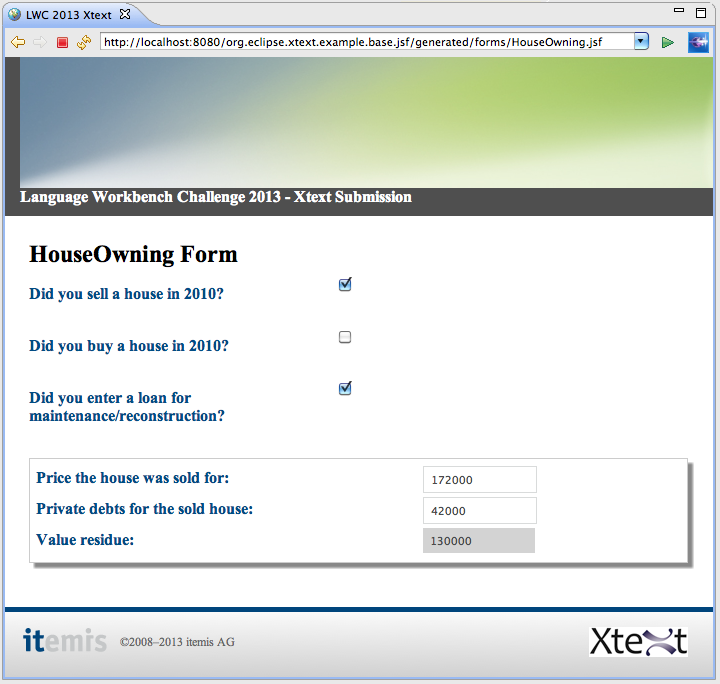
\includegraphics[width=15cm]{./images/chapter02/questionnaireApplication.png}
\end{center}
 
Now it's show time. You can modify your QL model and save it. The XHTML files
will be regenerated on the fly. The server needs some seconds to reload the
backing beans. Afterwards you can press the \emph{Refresh} button and see the
result immediately.
